\documentclass{beamer}

%\usepackage[utf8]{inputenc}
\usepackage{fontspec}
\usepackage{amsmath,amssymb,tikz-cd}
\usepackage{xcolor, xspace}

%\usefonttheme[onlymath]{serif}

\definecolor{darkblue}{HTML}{12335F}
\definecolor{myblue}{HTML}{00A2FF}

%--------------------------------------------------------------------------------
% Custom Template
%--------------------------------------------------------------------------------
\usecolortheme[named=myblue]{structure}

\setbeamertemplate{frametitle}{\vspace{5mm}\bfseries\insertframetitle}
\setbeamercolor{frametitle}{fg=darkblue}

\setbeamerfont{section in toc}{series=\bfseries}
\setbeamercolor{section in toc}{fg=darkblue}

\AtBeginEnvironment{theorem}{%
	\setbeamercolor{block title}{fg=white, bg=darkblue}
	\setbeamercolor{block body}{fg=black,bg=myblue!20}
}

\newcommand{\sectionSlide}[2]{
{
	\setbeamercolor{background canvas}{bg=darkblue}
	\begin{frame}
		\bfseries
		{\color{white}
			\huge {#1}
		}
		\vspace{5mm}

		{\color{myblue}
			{#2}
		}
	\end{frame}
	}
}

%--------------------------------------------------------------------------------
% Custom Commands
%--------------------------------------------------------------------------------
\newcommand{\ang}[1]{\langle #1 \rangle}
\newcommand{\warn}[1]{\textbf{\color{red}#1}}
\newcommand{\ER}{Erd\H{o}s R\'enyi\xspace}
\newcommand{\BF}{Bohman-Frieze\xspace}
\newcommand{\nl}{
\vspace{5mm}

}

%--------------------------------------------------------------------------------
% Fonts
%--------------------------------------------------------------------------------
\setmainfont{Baskerville}
%\setsansfont{Graphik}
\setsansfont{Baskerville}

\begin{document}

%--------------------------------------------------------------------------------
% Title Page
%--------------------------------------------------------------------------------
{
\setbeamercolor{background canvas}{bg=darkblue}
\begin{frame}
	\bfseries
	{\color{white}
		\huge Percolation Phase Transitions on Dynamically Grown Graphs
	}
	\vspace{5mm}

	{\color{myblue}
		\large Braden Hoagland

		Advised by Rick Durrett
	}

	\vspace*{\fill}
	{\color{white}
		\small April 15, 2022
	}
\end{frame}
}

%--------------------------------------------------------------------------------
% Background
%--------------------------------------------------------------------------------
\section{Background}
\sectionSlide{Background}{Dynamically grown graphs and percolation}

\begin{frame}{Dynamically Grown Graphs}
	
	Start with a graph with $n$ vertices and 0 edges \nl

	Add edges randomly every $1/n$ units of time \nl

	We'll work in the limit as $n\to \infty$
\end{frame}

\begin{frame}{Dynamically Grown Graphs}
        \begin{figure}[H]
                \centering
                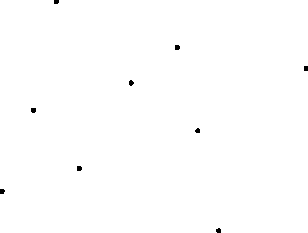
\includegraphics[scale=1]{fig/graph-1.pdf}
        \end{figure}
\end{frame}
\begin{frame}{Dynamically Grown Graphs}
        \begin{figure}[H]
                \centering
                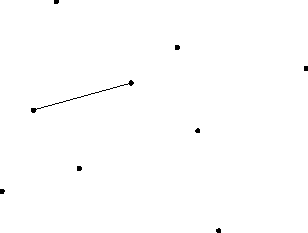
\includegraphics[scale=1]{fig/graph-2.pdf}
        \end{figure}
\end{frame}
\begin{frame}{Dynamically Grown Graphs}
        \begin{figure}[H]
                \centering
                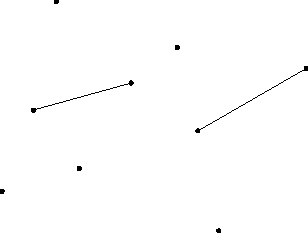
\includegraphics[scale=1]{fig/graph-3.pdf}
        \end{figure}
\end{frame}
\begin{frame}{Dynamically Grown Graphs}
        \begin{figure}[H]
                \centering
                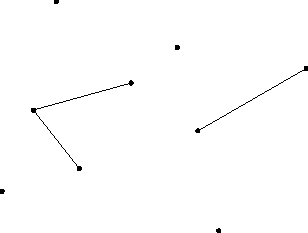
\includegraphics[scale=1]{fig/graph-4.pdf}
        \end{figure}
\end{frame}
\begin{frame}{Dynamically Grown Graphs}
        \begin{figure}[H]
                \centering
                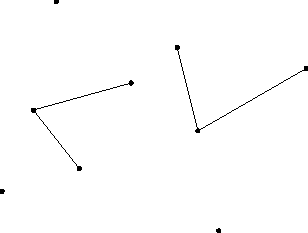
\includegraphics[scale=1]{fig/graph-5.pdf}
        \end{figure}
\end{frame}

\begin{frame}{Percolation}
	
	A \emph{giant component} is a cluster that takes up a finite fraction of the graph \nl

	\emph{Percolation} is when a giant component first emerges (call this time $t_c$) \nl

	\pause
	This emergence has lots of different behaviors
\end{frame}

\begin{frame}{\ER}
	\begin{figure}[H]
		\centering
		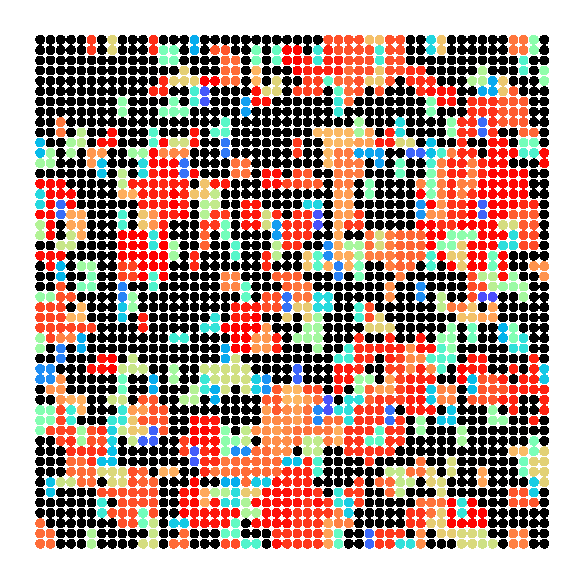
\includegraphics[scale=0.7]{fig/precrit.pdf}
		%\caption{}
	\end{figure}
\end{frame}
\begin{frame}{\ER}
        \begin{figure}[H]
                \centering
                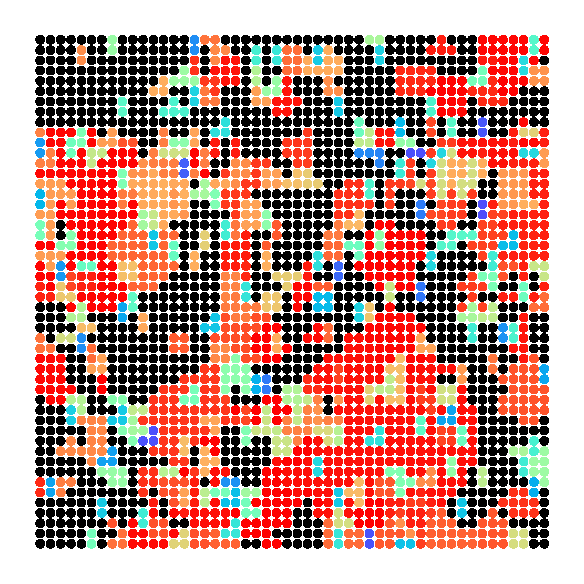
\includegraphics[scale=0.7]{fig/crit.pdf}
                %\caption{}
        \end{figure}
\end{frame}
\begin{frame}{\ER}
        \begin{figure}[H]
                \centering
                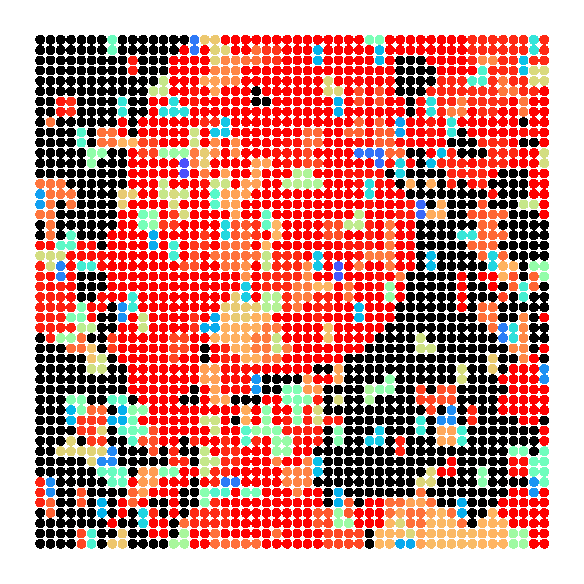
\includegraphics[scale=0.7]{fig/postcrit.pdf}
                %\caption{}
        \end{figure}
\end{frame}

\begin{frame}{da Costa}
        \begin{figure}[H]
                \centering
                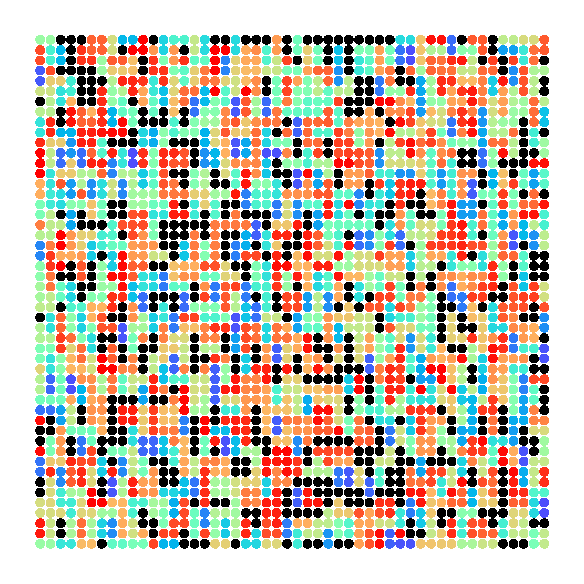
\includegraphics[scale=0.7]{fig/exp-precrit.pdf}
                %\caption{}
        \end{figure}
\end{frame}
\begin{frame}{da Costa}
        \begin{figure}[H]
                \centering
                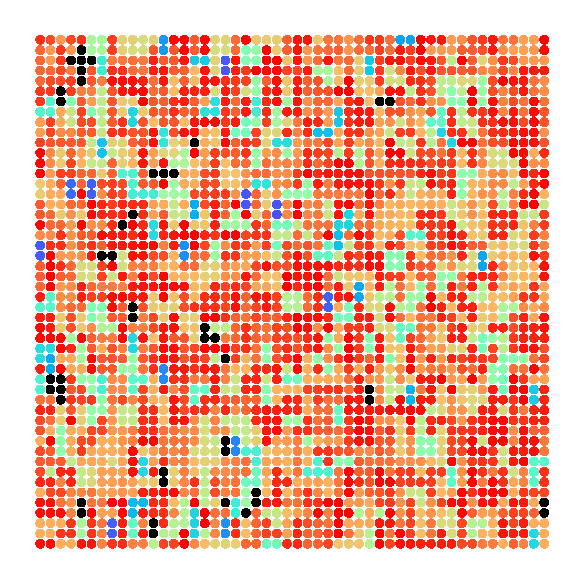
\includegraphics[scale=0.7]{fig/exp-crit.pdf}
                %\caption{}
        \end{figure}
\end{frame}
\begin{frame}{da Costa}
        \begin{figure}[H]
                \centering
                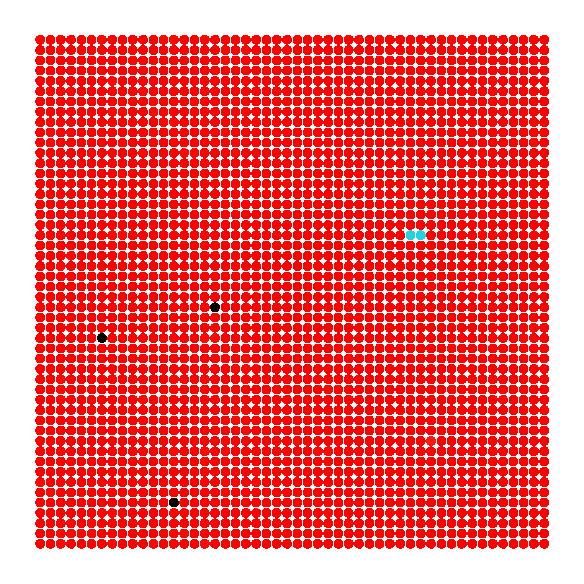
\includegraphics[scale=0.7]{fig/exp-postcrit.pdf}
                %\caption{}
        \end{figure}
\end{frame}

\begin{frame}{Explosive Percolation}

	\emph{Explosive Percolation} is a sudden, seemingly discontinuous emergence of the giant component
\end{frame}

%--------------------------------------------------------------------------------
% Basic Results
%--------------------------------------------------------------------------------
\section{Basic Results}
\sectionSlide{Basic Results}{Continuous phase transition and scaling behavior}

\begin{frame}{Continuous phase transition}

	\emph{Achlioptas rule}: select two edges at random, then choose one of them to keep via some rule based on the cluster sizes of the edges' vertices \nl

	Achlioptas (2009): claimed to have found a discontinuous emergence of a giant component based on simulations
\end{frame}

\begin{frame}{Continuous phase transition}

	Riordan and Warnke (2012) \nl

	\emph{$\ell$-vertex rule}: choose $\ell$ vertices i.i.d., and you're only required to add an edge if all $\ell$ of them are in distinct clusters (generalizes Achlioptas processes) \nl

        All $\ell$-vertex rules have a continuous phase transition \nl

        \pause
        Proof by contradiction...
\end{frame}

\begin{frame}{Scaling behavior}

	Because of the continuous phase transition, the distribution of vertices belonging to a cluster of size $s$ follows a power law
	\[
	s^{1-\tau} f \, (s \delta^{1/\sigma})
	\] 
	where $\delta = t - t_c$ and $\,f\,$ is a scaling function. \nl

	\pause
	Noticing scaling behavior in rules with explosive percolation was motivation for proving their continuity
\end{frame}

\begin{frame}{Critical Exponents}

	\warn{Hi}
\end{frame}


%--------------------------------------------------------------------------------
% Two-Choice Rules
%--------------------------------------------------------------------------------
\section{Two-Choice Rules}
\sectionSlide{Two-Choice Rules}{Our Results}

\begin{frame}{Two-Choice Rules}

	Pick two finite groups of i.i.d. vertices \nl

	Follow a deterministic method to choose a representative vertex from each group (can be a different rule for each group) \nl

	Add an edge between the two representatives
\end{frame}

\begin{frame}{Two-Choice Rules}
	
	\ER: Both groups are size 1, so this is the same as sampling edges randomly \nl

	Correspondence with \ER random graph \nl

	\pause
	da Costa: both groups are of size $m$, and pick the vertex with the smallest cluster size from each group
\end{frame}

\begin{frame}{Scaling Relations}
	
	Consider
	\[
	1 - \ang{1}_{\phi} = 1 - \sum_{s \text{ finite}} \phi(s),
	\] where $\phi(s) = \mathbb{P}( \text{representative has cluster size } s )$ \nl

	Under certain regularity conditions, this quantity is $\sim \delta^{F(\beta)}$ \warn{need to define $\sim$} \nl

	\pause
	Can express critical exponents in terms of $\beta$ and $F(\beta)$
\end{frame}

\begin{frame}{Scaling Relations}

	\warn{need to introduce $\gamma_{\phi}$ somewhere}

	For a two-choice rule with $1 - \ang{1}_{\phi} \sim \delta^{F(\beta)}$,

	\begin{align*}
		\gamma_{\phi} &= F(\beta) - \beta + 1 \\
		\gamma_{P} &= 2 (F(\beta) - \beta) + 1 \\
		\frac{1}{\sigma} &= 2 F(\beta) - \beta + 1 \\
		\tau &= \frac{\beta}{2 F(\beta) - \beta + 1} +2
	\end{align*}
	
\end{frame}

\begin{frame}{da Costa}
	
	da Costa (2015): if groups are size $m$ and the rule selects the vertex with the smallest cluster size, then
	\begin{align*}
		\gamma_{\phi} &= 1 + (m-1)\beta \\
		\gamma_{P} &= 1 + 2(m-1)\beta \\
		\frac{1}{\sigma} &= 1 + (2m-1)\beta \\
		\tau &= 2 + \frac{\beta}{1 + (2m-1)\beta} 
	\end{align*}
\end{frame}

\begin{frame}{da Costa}
	\warn{need to introduce $S$ somewhere}

	Since $1 - \ang{1}_{\phi}$ is the probability that a vertex chosen by our rule is in an infinite cluster,
	\[
	1 - \ang{1}_{\phi} = S^{\,m} \sim (\delta^{\beta})^{m} \sim \delta^{m \beta},
	\] 
	so $F(\beta) = m\beta$ \nl

	Plugging this into our earlier equations recovers da Costa's scaling relations
\end{frame}

\begin{frame}{\ER}
	
	This is the da Costa rule with $m=1$, so
	\begin{align*}
		\gamma_{\phi} = \gamma_{P} &= 1 \\
		\frac{1}{\sigma} &= \beta + 1 \\
		\tau &= \frac{\beta}{\beta + 1} + 2
	\end{align*}
	
\end{frame}

\begin{frame}{\ER}
	
	Much more is possible since \ER is such a simple rule \nl

	Known result: $\beta = 1$, i.e. giant component grows linearly near $t_{c}$ \nl

	This fixes $\gamma_{P} = 1, \quad \frac{1}{\sigma} = 2, \quad \tau = 5/2$
\end{frame}

\begin{frame}{\ER ($n =2500$)}

	\begin{figure}[H]
		\centering
		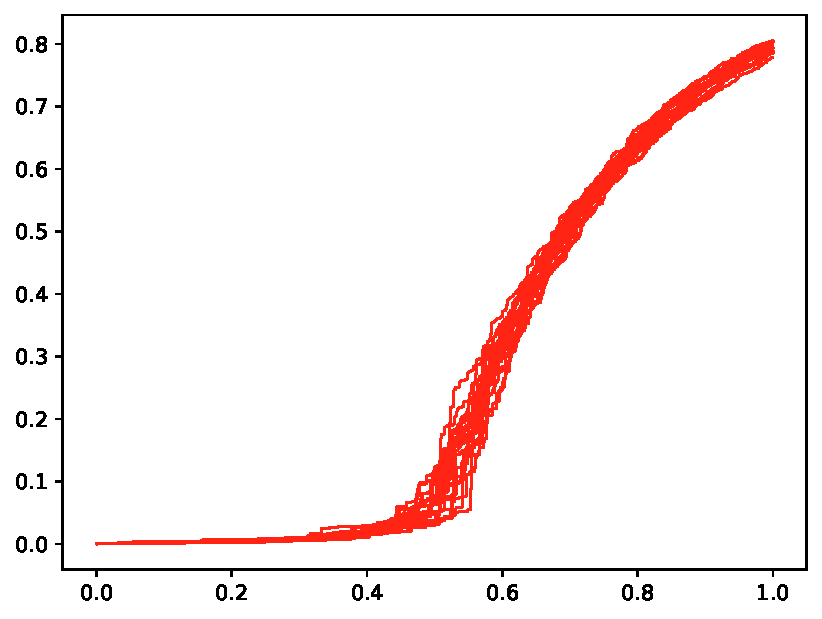
\includegraphics[scale=0.7]{fig/2500.pdf}
	\end{figure}
\end{frame}

\begin{frame}{\ER}
	
	Scaling behavior occurs in region of order $\Theta(s^{-1/2})$ around $t_{c}$ \nl

	As $s \to \infty$, the scaling window shrinks \nl

	In particular, the region of linear giant component growth shrinks as $n \to \infty$

\end{frame}

\begin{frame}{\ER ($n =100$)}

        \begin{figure}[H]
                \centering
                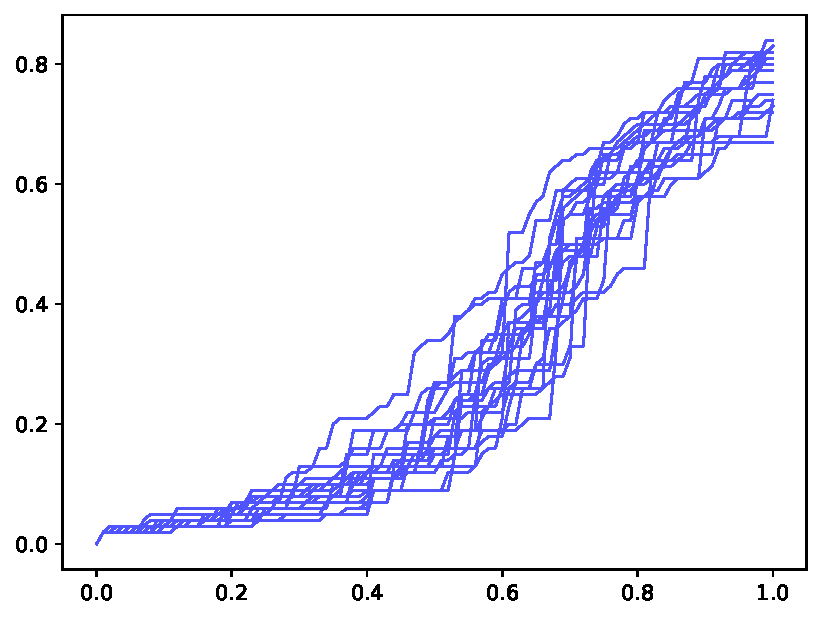
\includegraphics[scale=0.7]{fig/100.pdf}
        \end{figure}
\end{frame}
\begin{frame}{\ER ($n =1000$)}

        \begin{figure}[H]
                \centering
                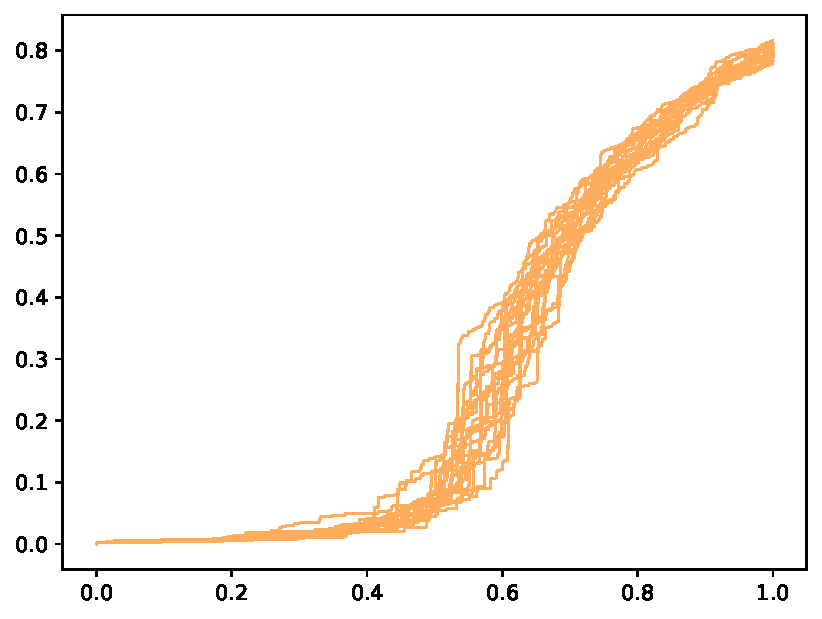
\includegraphics[scale=0.7]{fig/1000.pdf}
        \end{figure}
\end{frame}
\begin{frame}{\ER ($n =2500$)}

        \begin{figure}[H]
                \centering
                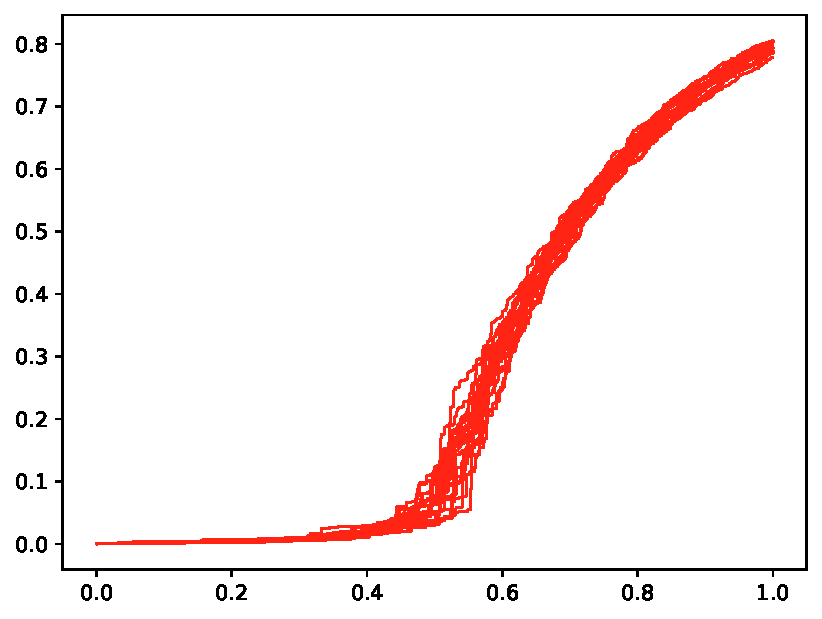
\includegraphics[scale=0.7]{fig/2500.pdf}
        \end{figure}
\end{frame}

%--------------------------------------------------------------------------------
% Bounded Size Rules
%--------------------------------------------------------------------------------
\section{Bounded Size Rules}
\sectionSlide{Bounded Size Rules}{Rules that are almost \ER}

\begin{frame}{Bounded Size Rules}
	
	A \emph{bounded size rule} with size threshold $K$ treats all clusters of size $> K$ the same \nl

	Intuition: eventually there will be so few clusters of size $\leq K$ that it starts acting like \ER \nl
\end{frame}

\begin{frame}{\BF}
	
	For each group of vertices, do the following:
	\begin{itemize}
		\item Pick $m+1$ vertices
		\item If any of the first $m$ vertices are isolated, pick one at random as the representative
		\item If not, pick the $(m+1)$-st vertex instead
	\end{itemize} \nl

	Bounded size rule with size threshold $K = 1$
\end{frame}

\begin{frame}{Scaling Relations}
	
	For any bounded size rule, $1 - \ang{1}_{\phi} \sim \delta^{\beta}$ \nl

	Thus $F(\beta) = \beta$ (the same as \ER!) \nl

	Same scaling relations as \ER (with potentially different $\beta$)
	\begin{align*}
                \gamma_{\phi} = \gamma_{P} &= 1 \\
                \frac{1}{\sigma} &= \beta + 1 \\
                \tau &= \frac{\beta}{\beta + 1} + 2
        \end{align*}
\end{frame}

\begin{frame}
	
	\warn{Need to finish up the presentation somehow}
\end{frame}



\end{document}
